\chapter{Metode Penelitian}

\section{Alat dan Bahan Tugas Akhir}

\subsection{Alat Tugas Akhir}

\begin{enumerate}
    \item Perangkat komputer, baik \textit{desktop} maupun komputer jinjing (\textit{laptop}), sebagai \textbf{komputer utama} dengan
    \begin{itemize}
        \item sistem operasi Windows 11 Home, Pro, atau SKU lain yang mendukung kapabilitas Windows Subsystem for Linux versi 2 (WSL2);
        \item arsitektur x86\_64 (64-bit) dengan prosesor seri Intel Core generasi ke-8 atau lebih tinggi;
        \item memori (RAM) minimal 8 GB; dan
        \item ruang penyimpanan minimal 64 GB.
    \end{itemize} Bila menggunakan \textit{virtual machine}, harap pastikan fungsionalitas "\textit{nested virtualization}" bekerja dengan baik karena Windows Subsystem for Linux versi kedua (WSL2) membutuhkan dukungan virtualisasi. Pada tugas akhir ini, digunakan perangkat komputer \textit{all-in-one} ASUS seri ZN270IE beridentitas "COM25" di Laboratorium Jaringan Komputer dan Aplikasi Terdistribusi, Departemen Teknik Elektro dan Teknologi Informasi, Universitas Gadjah Mada dengan detail sebagai berikut.
    \begin{itemize}
        \item Sistem operasi Windows 11 Pro (versi 22H2) 64-bit
        \item Prosesor Intel Core i7-7700T dengan kecepatan 2,90 GHz dan arsitektur x86\_64 (64-bit)
        \item Memori (RAM) sebanyak 16 GB
        \item Kemampuan layar sentuh dengan multisentuh hingga sepuluh jari secara bersamaan
    \end{itemize}

    \item Perangkat lunak "Windows Subsystem for Linux 2 (WSL2)" versi perilisan terbaru yang terinstal pada komputer utama. Untuk menginstal WSL2 serta distribusi Linux \textit{default}-nya atau memastikan keterbaruan versi WSL yang telah terinstal, jalankan perintah berikut pada PowerShell atau Command Prompt.
    \begin{lstlisting}
wsl --install\end{lstlisting}
    Apabila terdapat perangkat lunak \textit{virtual machine} pihak ketiga (VirtualBox, VMware, dan sebagainya) yang terinstal pada komputer utama tersebut, harap pastikan bahwa perangkat lunak \textit{virtual machine} tersebut telah diperbarui ke versi paling baru dan kompatibel dengan WSL2 atau Hyper-V (kapabilitas yang menenagai WSL2); instalasi WSL2 dan perangkat lunak \textit{virtual machine} pihak ketiga tersebut dalam sistem yang sama dapat menyebabkan degradasi performa pada perangkat lunak \textit{virtual machine} pihak ketiga tersebut karena perangkat lunak \textit{virtual machine} pihak ketiga tersebut mencoba mengakomodasi aktifnya kapabilitas Hyper-V.

    \item Perangkat komputer bersistem operasi Ubuntu 22.04 (LTS) sebagai \textbf{komputer referensi (\textit{reference machine})}. Perangkat komputer dapat berupa komputer \textit{desktop} ataupun komputer jinjing (\textit{laptop}). Apabila tidak memungkinkan, mesin referensi dapat disubstitusikan dengan \textit{virtual machine} yang berjalan di suatu perangkat komputer \textit{host} melalui perangkat lunak \textit{virtual machine}. Pada tugas akhir ini, penulis menggunakan \textit{virtual machine} yang menjalankan sistem operasi Ubuntu 22.04 (LTS) melalui perangkat lunak virtualisasi "UTM" dengan \textit{host} komputer jinjing Apple MacBook Air keluaran tahun 2020 (berprosesor M1) bersistem operasi macOS 13 "Ventura".

    \item Perangkat lunak untuk keperluan pengembangan (semuanya diinstal di lingkungan Windows):
    \begin{enumerate}
        \item Microsoft Visual Studio Code (versi terbaru)
        \item Python versi 3.11 atau lebih baru dengan sejumlah pustaka (\textit{library}) pihak ketiga yang terinstal (menggunakan \verb|pip|):
        \begin{enumerate}
            \item \verb|dbus-next|
            \item \verb|winsdk|
        \end{enumerate}
    \end{enumerate}
    
    \item Perangkat lunak untuk keperluan pengujian akhir (semuanya diinstal di dalam WSL):
    \begin{enumerate}
        \item Spotify
        \item Mozilla Thunderbird
        \item Google Chrome
    \end{enumerate}
\end{enumerate}

\subsection{Bahan Tugas Akhir}

Dalam pengerjaan tugas akhir ini, digunakan sejumlah dokumen standar atau spesifikasi yang berkaitan dengan protokol atau perangkat lunak yang digunakan. Berikut dokumen-dokumen yang dimaksud.
\begin{enumerate}
    \item Dokumen spesifikasi D-Bus \cite{dbus-specification}
    \item Dokumen spesifikasi FreeDesktop (XDG) Desktop Notifications \cite{xdg-desktop-notifications-specification}
    \item Dokumen spesifikasi FreeDesktop (XDG) Media Player Remote Interfacing Specification (MPRIS) \cite{xdg-mpris-specification}
\end{enumerate}


\section{Alur Tugas Akhir}

Guna menciptakan arah penelitian yang terstruktur, ditentukan alur pelaksanaan tugas akhir di bawah ini. Tahap-tahap yang tertera di sini merupakan penjabaran lebih lanjut dari tujuan-tujuan penelitian yang telah ditentukan. Gambar \ref{diagram-alir-pelaksanaan} menunjukkan alur pelaksanaan tugas akhir dalam bentuk diagram alir (\textit{flowchart}) dan Tabel \ref{tabel-agenda-pelaksanaan} menjelaskan perencanaan agenda pelaksanaan tahap-tahap ini.

\begin{enumerate}
    \item \textbf{Pemeriksaan fungsionalitas penanganan notifikasi dan kontrol media di Windows Subsystem for Linux (WSL)}\\
    Pertama-tama, dilakukan pemeriksaan terlebih dahulu mengenai kedua aspek yang akan dibahas dalam tugas akhir ini, yakni aspek penanganan notifikasi (\textit{notification handling}) dan aspek kontrol media (\textit{media control}). Hal ini dilakukan guna memvalidasi alasan utama yang melatarbelakangi tugas akhir ini, yakni ketiadaan dukungan penanganan notifikasi dan kontrol media di Windows Subsystem for Linux (WSL).

    \item \textbf{Analisis \textit{behavior} penanganan notifikasi dan kontrol media pada instalasi sistem operasi Linux sungguhan sebagai basis implementasi di Windows Subsystem for Linux (WSL)}\\
    Dilakukan analisis kedua aspek utama yang dibahas dalam tugas akhir ini, penanganan notifikasi dan kontrol media, pada sistem operasi Linux sungguhan yang terinstal di komputer referensi. Pada tahap ini, dilakukan investigasi tentang bagaimana sistem D-Bus berperan dalam pencapaian kedua aspek tersebut. Guna meminimalkan perbedaan yang dapat terjadi, sistem operasi Linux sungguhan yang terinstal menggunakan distribusi yang sama dengan distribusi \textit{default} pada WSL, yakni Ubuntu (versi 22.04 pada waktu penyusunan tugas akhir ini).

    \item \textbf{Penyesuaian konfigurasi Windows Subsystem for Linux untuk mendukung perangkat lunak FancyWSL}\\
    Secara \textit{default}, instalasi Windows Subsystem for Linux (WSL) tidak bisa langsung dihubungkan dengan perangkat lunak FancyWSL yang akan dikembangkan; diperlukan sejumlah modifikasi terlebih dahulu pada sejumlah konfigurasi di WSL, yakni pemastian penggunaan systemd sebagai sistem init dan pengaturan \textit{daemon} D-Bus agar menerima penghubungan melalui TCP.

    \item \textbf{Analisis kesamaan antarmuka FreeDesktop Desktop Notifications di Linux dengan ToastNotification di Windows}\\
    Guna menghubungkan ekosistem penanganan notifikasi WSL dengan ekosistem penanganan notifikasi Windows, diperlukan analisis mendalam pada detail implementasi penanganan notifikasi pada masing-masing platform (Linux dan Windows) dan pencocokan antarmuka keduanya agar dapat dihubungkan.

    \item \textbf{Analisis kesamaan antarmuka Media Player Remote Interfacing Specification (MPRIS) di Linux dengan System Media Transport Controls (SMTC) di Windows}\\
    Guna menghubungkan ekosistem pengontrolan media WSL dengan ekosistem pengontrolan media Windows, diperlukan analisis mendalam pada detail implementasi sistem pengontrolan media pada masing-masing platform (Linux dan Windows) dan pencocokan antarmuka keduanya agar dapat dihubungkan.

    \item \textbf{Pengembangan perangkat lunak FancyWSL}\\
    Pada tahap ini, dilakukan pengembangan perangkat lunak FancyWSL dari awal hingga akhir. Mengingat perangkat lunak ini mencakup sejumlah fungsi yang cukup luas, tahap ini dibagi kembali menjadi empat subtahap sebagai berikut.
    \begin{enumerate}
        \item \textbf{Pengembangan tahap awal: Penghubungan dengan D-Bus dan pengimplementasian aspek \textit{persistence} (\textit{daemon})}\\
        Subtahap ini mulai mengeksplorasi langkah-langkah penghubungan perangkat lunak FancyWSL dengan bus perpesanan D-Bus (bus sesi atau \textit{session bus}) yang berjalan di WSL.
        
        \item \textbf{Pengembangan fungsi penanganan notifikasi}\\
        Subtahap ini mengimplementasikan mekanisme penangkapan notifikasi dari perangkat-perangkat lunak yang berjalan di WSL, mekanisme penampilan notifikasi secara \textit{native} di lingkungan Windows dengan menggunakan ToastNotification, serta mekanisme penghubungan keduanya.

        \item \textbf{Pengembangan fungsi kontrol media}\\
        Subtahap ini mengimplementasikan mekanisme pemantauan media yang sedang terputar pada perangkat-perangkat lunak di WSL, mekanisme penampilan elemen kontrol media System Media Transport Controls di Windows, serta mekanisme penghubungan keduanya.

        \item \textbf{Pengimplementasian \textit{guards} tambahan}\\
        Subtahap ini mengimplementasikan pemeriksaan-pemeriksaan yang bersifat "\textit{nice to have}" yang umumnya tidak bersifat \textit{mandatory} pada perangkat-perangkat lunak level \textit{proof-of-concept} (PoC) namun bersifat \textit{mandatory} pada perangkat-perangkat lunak level \textit{production}, seperti pemeriksaan platform tempat perangkat lunak FancyWSL dijalankan, pemeriksaan kapabilitas pada WSL yang diperlukan oleh FancyWSL (keberadaan perangkat lunak WSL di Windows, versi WSL pada distribusi \textit{default} yang terinstal di WSL, ketersediaan sistem init systemd, dan lain-lain)
    \end{enumerate}

    \item \textbf{Pengintegrasian FancyWSL dengan \textit{lifecycle} Windows Subsystem for Linux (WSL)}\\
    Guna menciptakan pengalaman pengguna (\textit{user experience}) yang lebih \textit{seamless}, dapat dilakukan pengintegrasian perangkat lunak FancyWSL lebih lanjut dengan WSL dengan cara menghubungkan pemulaian FancyWSL dengan \textit{startup} WSL.
\end{enumerate}

\begin{figure}
    \centering
    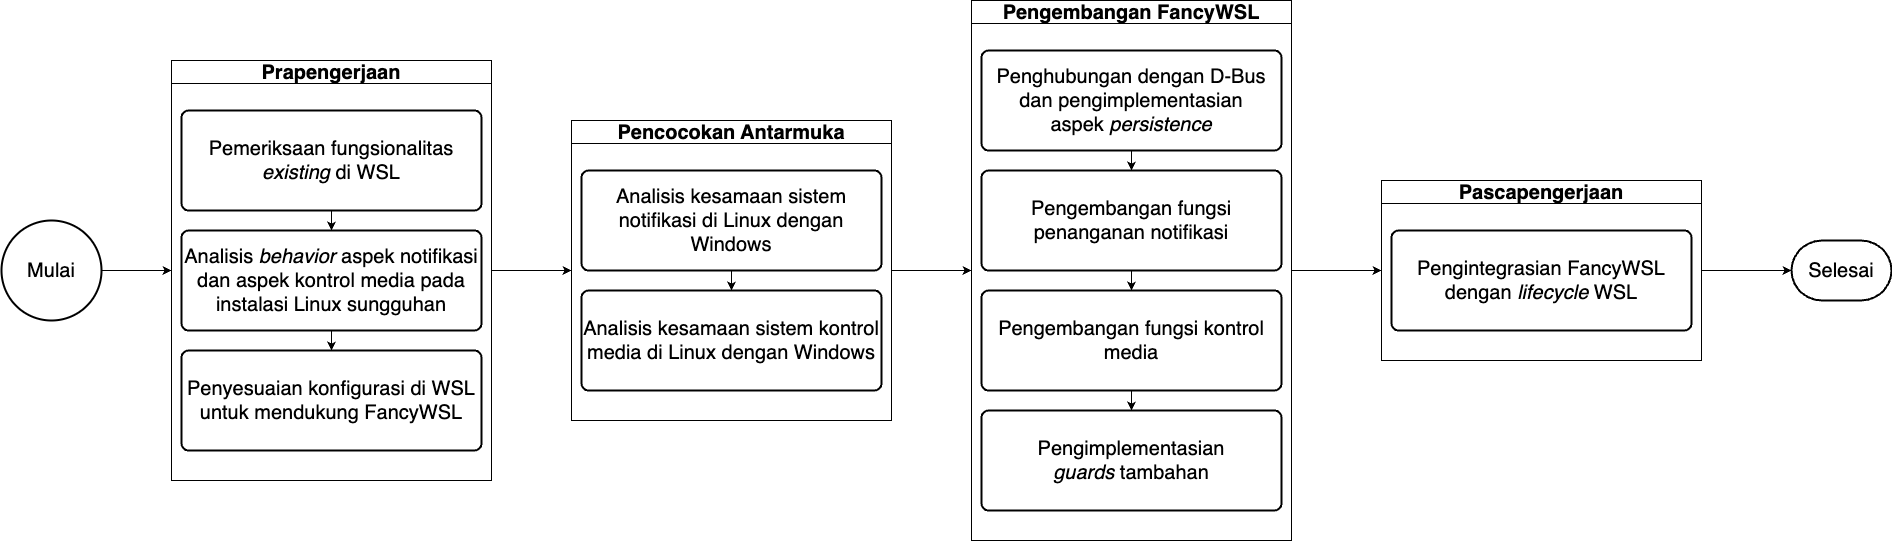
\includegraphics[width=1\linewidth]{assets/alur-pengerjaan-v1.png}
    \caption{Diagram alir (\textit{flowchart}) pelaksanaan tugas akhir}
    \label{diagram-alir-pelaksanaan}
\end{figure}

\begin{table}
    \centering
    \caption{Agenda pelaksanaan tugas akhir per minggu (\textit{week})}
    \begin{tabular}{|c|p{4cm}|c|c|c|c|c|c|c|c|} \hline 
        \multirow{3}{*}{\textbf{No.}} & \multirow{3}{*}{\textbf{Tahap}} & \multicolumn{8}{c|}{\textbf{2023}}\\ \cline{3-10} 
        & & \multicolumn{4}{c|}{\textbf{Oktober}} & \multicolumn{4}{c|}{\textbf{November}}\\ \cline{3-10} 
        & & \textbf{W1} & \textbf{W2} & \textbf{W3} & \textbf{W4} & \textbf{W1} & \textbf{W2} & \textbf{W3} & \textbf{W4}\\ \hline 
        1 & Pemeriksaan fungsionalitas di WSL & \cellcolor{black} &  &  &  &  &  &  & \\ \hline 
        2 & Analisis pada sistem operasi Linux sungguhan & \cellcolor{black} & \cellcolor{black} &  &  &  &  &  & \\ \hline 
        3 & Penyesuaian konfigurasi WSL untuk mendukung perangkat lunak FancyWSL &  &  & \cellcolor{black} & \cellcolor{black} &  &  &  & \\ \hline 
        4 & Analisis kesamaan antarmuka notifikasi &  &  & \cellcolor{black} & \cellcolor{black} & \cellcolor{black} & &  & \\ \hline 
        5 & Analisis kesamaan antarmuka pengontrolan media &  &  & \cellcolor{black} & \cellcolor{black} & \cellcolor{black} &  &  & \\ \hline 
        6 & Pengembangan perangkat lunak FancyWSL &  &  &  &  & \cellcolor{black} & \cellcolor{black} & \cellcolor{black} & \cellcolor{black}\\ \hline 
        7 & Pengintegrasian FancyWSL dengan \textit{lifecycle} WSL &  &  &  &  &  &  &  & \cellcolor{black}\\ \hline 
    \end{tabular}
    \label{tabel-agenda-pelaksanaan}
\end{table}

\section{Metode yang Digunakan}

Sesuai dengan analisis perbandingan metode yang telah dibahas di Bab II, tugas akhir ini menggunakan metode penghubungan lingkungan Windows Subsystem for Linux (WSL) dengan lingkungan \textit{host} Windows dengan memperluas cakupan koneksi bus perpesanan D-Bus yang berjalan di dalam WSL sehingga dapat dicapai oleh perangkat lunak FancyWSL yang berjalan di sisi Windows. Oleh karena itu, secara garis besar, metode tugas akhir ini dilakukan adalah dengan
\begin{enumerate}
    \item mengembangkan satu buah perangkat lunak bernama FancyWSL yang berjalan di lingkungan \textit{host} Windows dan
    \item melakukan sejumlah konfigurasi yang diperlukan di Windows Subsystem for Linux (WSL) agar dapat terhubung dengan perangkat lunak yang dikembangkan pada poin (1).
\end{enumerate}

\section{Metode Analisis Data}

Proses pengimplementasian akan dilakukan berdasarkan standar dan spesifikasi teknologi-teknokogi yang digunakan dalam tugas akhir ini. Sebagai contoh, pengimplementasian mekanisme komunikasi dengan D-Bus dilakukan dengan mengacu pada spesifikasi D-Bus \cite{dbus-specification}, pengimplementasian kapabilitas penanganan notifikasi dilakukan dengan mengacu pada FreeDesktop Desktop Notifications Specification \cite{xdg-desktop-notifications-specification}, dan pengimplementasian kapabilitas kontrol media dilakukan dengan mengacu pada standar Media Player Remote Interfacing Specification (MPRIS) \cite{xdg-mpris-specification}.

Pada akhir penelitian, akan dilakukan pengujian akhir yang membandingkan kondisi penggunaan Windows Subsystem for Linux (WSL) tanpa solusi yang dikembangkan di tugas akhir ini (kondisi bawaan) dan dengan solusi yang dikembangkan di tugas akhir ini (kondisi telah dilengkapi dengan perangkat lunak FancyWSL serta konfigurasi-konfigurasi yang diperlukan). Kedua bagian pengujian ini akan dilakukan menggunakan set perangkat lunak yang sama, yakni
\begin{itemize}
    \item Spotify (pengujian kontrol media dan notifikasi) dan
    \item Google Chrome (pengujian notifikasi).
\end{itemize}
